\fancychapter{Results: Pirate Game}
\label{ap:d}

\section{$3$ Player Game}

\subsection{Simulation}
\begin{lstlisting}
function out = simulation3players(a_11,a_12,a_13,a_22,a_23)
%
%        IN:
%-- alocation proposal a_ij -i number of the player that proposes a_ij coins 
%   to player j
%-- Check variables and set to defaults
if exist('a_11','var')~=1, a_11=99; end
if exist('a_12','var')~=1, a_12=0; end
if exist('a_13','var')~=1, a_13=1; end
if exist('a_22','var')~=1, a_22=100; end
if exist('a_23','var')~=1, a_23=0; end



%   cooperate= [1 0;0 1]
C= eye(2);
%   defect= [0 1;1 0]
D= ones(2)-eye(2);
% coin matrix
H= [1/sqrt(2) 1i/sqrt(2);1i/sqrt(2) 1/sqrt(2)];



step=0.1;
t=0:step:pi;

prob= zeros(size(t),8);

% variation of the paremeter gamma (the entanglement in the system)
for i=0:step:pi


ini= cos(i/2)*kron([1 0]', kron([1 0]',[1 0]'))+1i*sin(i/2)*kron([0 1]', kron([0 1]',[0 1]'));
% alternative: ini = J*kron([1 0]', kron([1 0]',[1 0]'));

% entanglement matrix
J= expm(1i*(i/2)*kron([0 1;1 0],kron([0 1;1 0],[0 1;1 0])));
% conjugate transpose of the entanglement matrix
Jd= ctranspose( expm(1i*(i/2)*kron([0 1;1 0],kron([0 1;1 0],[0 1;1 0]))));

% % --- Strategies

%% CCC 
   fin = Jd*kron(C,kron(C,C))*ini;
   payofffunc(fin, a_11,a_12,a_13,a_22,a_23)
%% CCD 
  fin = Jd*kron(C,kron(C,D))*ini;
  payofffunc(fin, a_11,a_12,a_13,a_22,a_23)
%% CDC 
 fin = Jd*kron(C,kron(D,C))*ini;
 payofffunc(fin, a_11,a_12,a_13,a_22,a_23)
% 
%% DCC 
 fin = Jd*kron(C,kron(D,D))*ini;
 payofffunc(fin, a_11,a_12,a_13,a_22,a_23)

% %% CDD 
  fin = kron(C,kron(D,D))*ini
  
      %% CC
 fn= Jd*kron(H,kron(C,C))*fin;
 payofffunc(fn, a_11,a_12,a_13,a_22,a_23)
%     %% CD
    fn= Jd*kron(H,kron(C,D))*fin 
     payofffunc(fn, a_11,a_12,a_13,a_22,a_23)
%     %% DC
   fn= Jd*kron(H,kron(D,C))*fin;
    payofffunc(fn, a_11,a_12,a_13,a_22,a_23)
%     %% DD
    fn= Jd*kron(H,kron(D,D))*fin; 
    payofffunc(fn, a_11,a_12,a_13,a_22,a_23)
  
% %% DCD 
  fin = kron(D,kron(C,D))*ini
        %% CC
 fn= Jd*kron(H,kron(C,C))*fin;
 payofffunc(fn, a_11,a_12,a_13,a_22,a_23)
%     %% CD
    fn= Jd*kron(H,kron(C,D))*fin 
     payofffunc(fn, a_11,a_12,a_13,a_22,a_23)
%     %% DC
   fn= Jd*kron(H,kron(D,C))*fin;
    payofffunc(fn, a_11,a_12,a_13,a_22,a_23)
%     %% DD
    fn= Jd*kron(H,kron(D,D))*fin; 
    payofffunc(fn, a_11,a_12,a_13,a_22,a_23)
% %% DDC 
  fin = kron(D,kron(D,C))*ini
        %% CC
 fn= Jd*kron(H,kron(C,C))*fin;
 payofffunc(fn, a_11,a_12,a_13,a_22,a_23)
%     %% CD
    fn= Jd*kron(H,kron(C,D))*fin 
     payofffunc(fn, a_11,a_12,a_13,a_22,a_23)
%     %% DC
   fn= Jd*kron(H,kron(D,C))*fin;
    payofffunc(fn, a_11,a_12,a_13,a_22,a_23)
%     %% DD
    fn= Jd*kron(H,kron(D,D))*fin; 
    payofffunc(fn, a_11,a_12,a_13,a_22,a_23)
% %% DDD 
 fin = kron(D,kron(D,D))*ini
 
       %% CC
 fn= Jd*kron(H,kron(C,C))*fin;
 payofffunc(fn, a_11,a_12,a_13,a_22,a_23)
%     %% CD
    fn= Jd*kron(H,kron(C,D))*fin 
     payofffunc(fn, a_11,a_12,a_13,a_22,a_23)
%     %% DC
   fn= Jd*kron(H,kron(D,C))*fin;
    payofffunc(fn, a_11,a_12,a_13,a_22,a_23)
%     %% DD
    fn= Jd*kron(H,kron(D,D))*fin; 
    payofffunc(fn, a_11,a_12,a_13,a_22,a_23)


end
end

function [] = payofffunc(fin, a_11,a_12,a_13,a_22,a_23)
%payofffunc_player1(fin)
%   
%                Calculates the payoff for player 1
%              IN
%                   fin: final state
%  

%-- Check variables and set to defaults
if exist('a_11','var')~=1, a_11=99; end
if exist('a_12','var')~=1, a_12=0; end
if exist('a_13','var')~=1, a_13=1; end
if exist('a_22','var')~=1, a_22=100; end
if exist('a_23','var')~=1, a_23=0; end

u1= a_11*(norm(conj([1 1 1 0 1 0 0 0]').*fin))^2 -200*(norm(conj([0 0 0 1 0 1 1 1]').*fin))^2
% 
u2=  a_12*(norm(conj([1 1 1 0 1 0 0 0]').*fin))^2 +(0.5+a_22*(norm(conj([0 1 1 1 0 1 1 1]').*fin))^2 -200*(norm(conj([1 0 0 0 1 0 0 0]').*fin))^2)*(norm(conj([0 0 0 1 0 1 1 1]').*fin))^2
% 
u3=  a_13*(norm(conj([1 1 1 0 1 0 0 0]').*fin))^2 +(0.5+a_23*(norm(conj([0 1 1 1 0 1 1 1]').*fin))^2 +100.5*(norm(conj([1 0 0 0 1 0 0 0]').*fin))^2)*(norm(conj([0 0 0 1 0 1 1 1]').*fin))^2
   

    
end
\end{lstlisting}

\subsection{ Captain proposes $(99,0,1)$.}
 
\subsubsection{ Accepted proposal after 1 round of the game.}
\label{tabs:accepted99}

\begin{table}[ht]
\begin{center}

\begin{tabular}{cc}
  a)\putindeepbox[7pt]{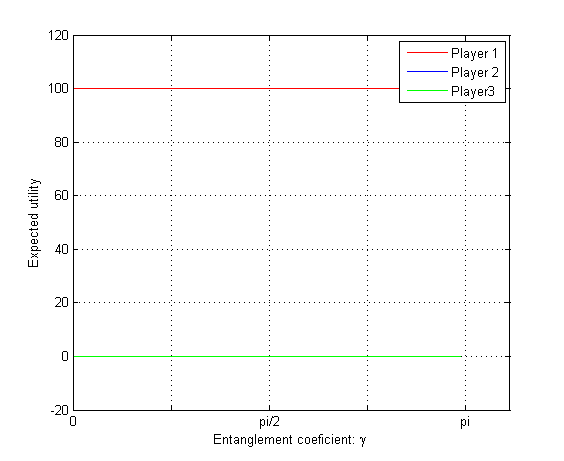
\includegraphics[scale=0.46]{3Accepted99/CCC.PNG}}
    & a1)\putindeepbox[7pt]{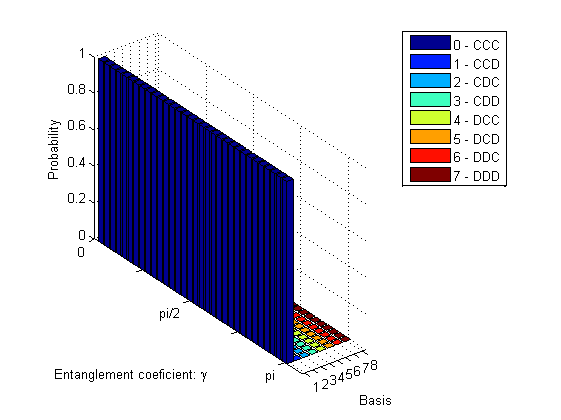
\includegraphics[scale=0.46]{3Accepted99/CCC_1.PNG}} \\
\end{tabular}
\caption{a) Expected utility for $3$ players, where the players will use the $(Cooperate, Cooperate, Cooperate)$ operators. The initial proposal is $(\alpha_{1}, \alpha_{2}, \alpha_{3}) =(99, 0, 1)$. a1) Probability distribution of the final state depending on the entanglement coefficient $\gamma$. }
\label{tab:3playerCCC99}
\end{center}
 \end{table}

\begin{table}[h]
\begin{center}
\begin{tabular}{cc}
  b)\putindeepbox[7pt]{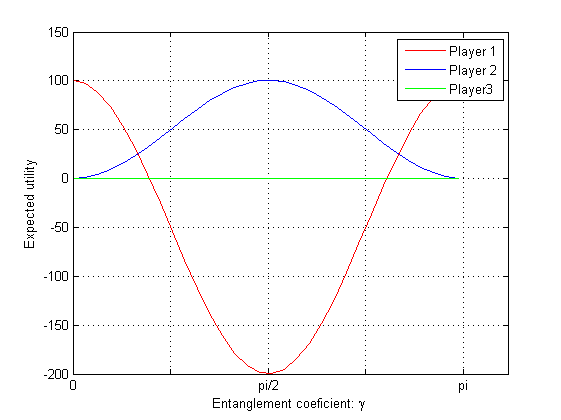
\includegraphics[scale=0.46]{3Accepted99/CCD.PNG}}
    & b1)\putindeepbox[7pt]{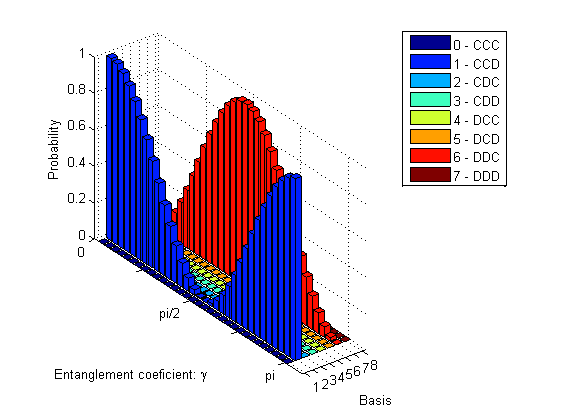
\includegraphics[scale=0.46]{3Accepted99/CCD_1.PNG}} \\
\end{tabular}
\caption{b) Expected utility for $3$ players, where the players will use the $(Cooperate, Cooperate, Defect)$ operators. b1) Probability distribution of the final state depending on the entanglement coefficient $\gamma$. }
\label{tab:3playerCCD99}
\end{center}
 \end{table}

\begin{table}[h]
\begin{center}
\begin{tabular}{cc}
  c)\putindeepbox[7pt]{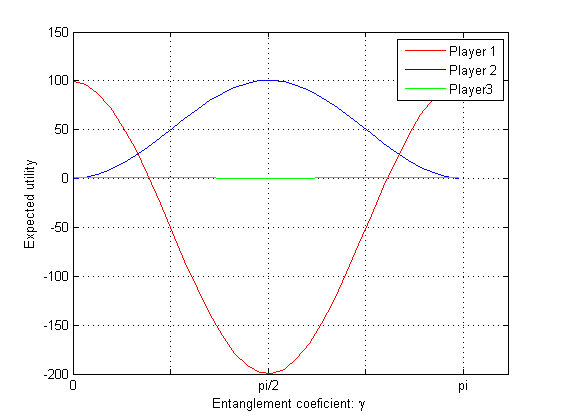
\includegraphics[scale=0.46]{3Accepted99/CDC.PNG}}
    & c1)\putindeepbox[7pt]{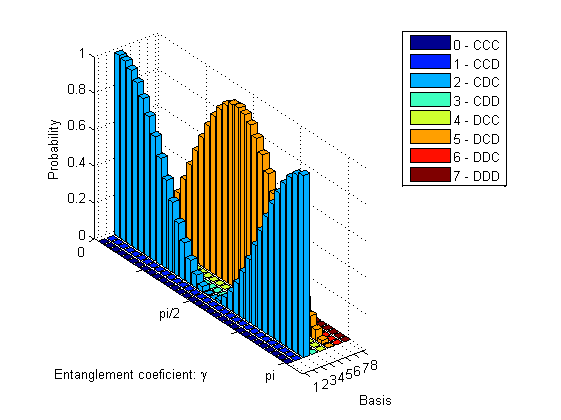
\includegraphics[scale=0.46]{3Accepted99/CDC_1.PNG}} \\
\end{tabular}
\caption{c) Expected utility for $3$ players, where the players will use the $(Cooperate, Defect, Cooperate)$ operators. c1) Probability distribution of the final state depending on the entanglement coefficient $\gamma$. }
\label{tab:3playerCDC99}
\end{center}
 \end{table}

\begin{table}[h]
\begin{center}
\begin{tabular}{cc}
  d)\putindeepbox[7pt]{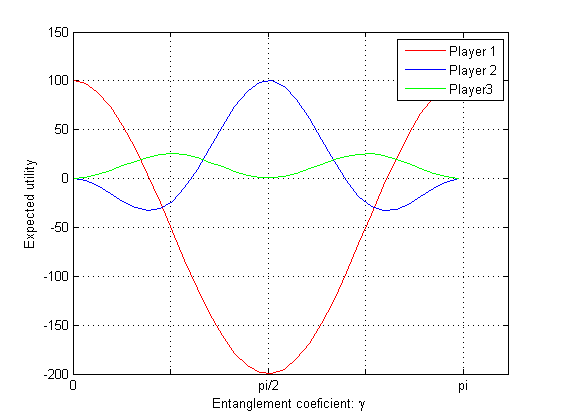
\includegraphics[scale=0.46]{3Accepted99/DCC.PNG}}
    & d1)\putindeepbox[7pt]{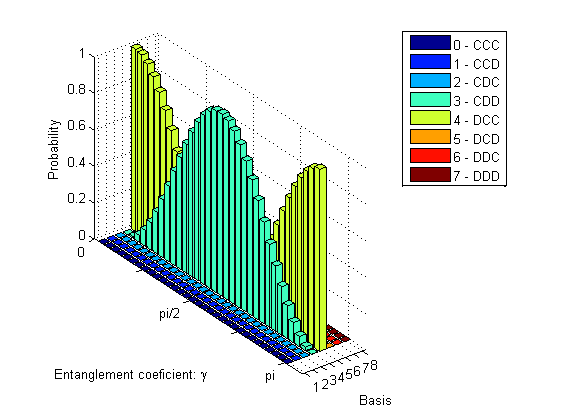
\includegraphics[scale=0.46]{3Accepted99/DCC_1.PNG}} \\
\end{tabular}
\caption{b) Expected utility for $3$ players, where the players will use the $(Defect, Cooperate, Cooperate)$ operators. b1) Probability distribution of the final state depending on the entanglement coefficient $\gamma$. }
\label{tab:3playerDCC99}
\end{center}
 \end{table}

\clearpage
\subsubsection{Initial proposal rejected; $(Cooperate , Defect, Defect)$}
\label{ap:d:CDD99}
%\item  Rejected proposal after 1 round of the game.\\

%\begin{itemize}

%\item In the first round the players use the operators $(CDD)$.\\

\begin{table}[h]
\begin{center}
\begin{tabular}{cc}
  a)\putindeepbox[7pt]{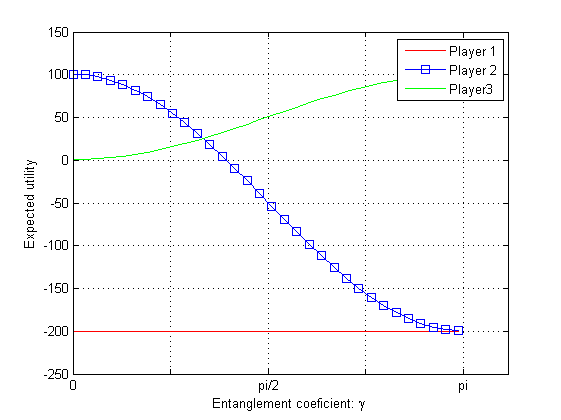
\includegraphics[scale=0.46]{3Rejected99/CDD_CC.PNG}}
    & a1)\putindeepbox[7pt]{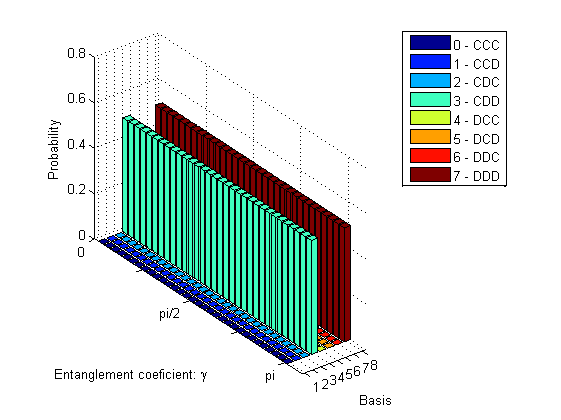
\includegraphics[scale=0.46]{3Rejected99/CDD_CC1.PNG}} \\
\end{tabular}
\caption{a) Expected utility for $3$ players, where the players will use the $(Cooperate , Defect, Defect)$ operators in the first round of the game; in the second round player 2 and player 3 will play $(CC)$. }
\label{tab:3playerCDD_CC99}
\end{center}
 \end{table}

\begin{table}[h]
\begin{center}
\begin{tabular}{cc}
  b)\putindeepbox[7pt]{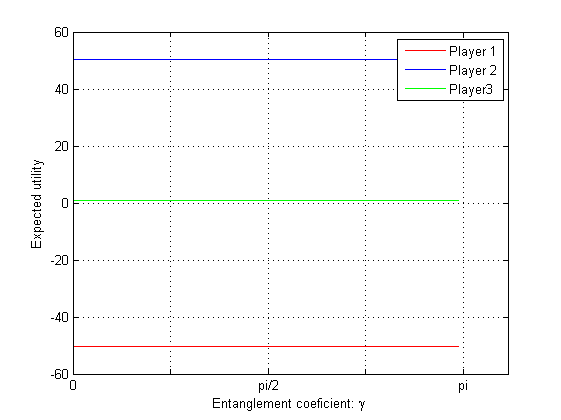
\includegraphics[scale=0.46]{3Rejected99/CDD_CD.PNG}}
    & b1)\putindeepbox[7pt]{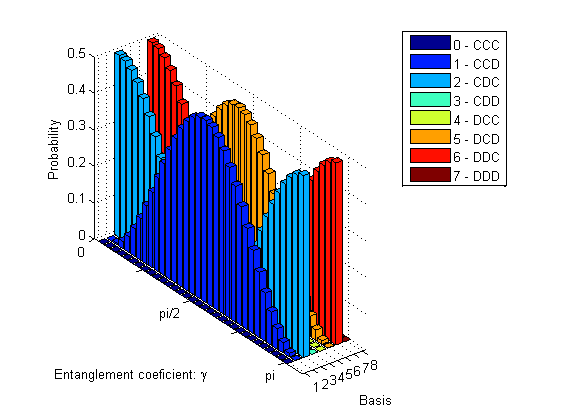
\includegraphics[scale=0.46]{3Rejected99/CDD_CD1.PNG}} \\
\end{tabular}
\caption{b) Expected utility for $3$ players, where the players will use the $(Cooperate , Defect, Defect)$ operators in the first round of the game; in the second round player 2 and player 3 will play $(CD)$. }
\label{tab:3playerCDD_CD99}
\end{center}
 \end{table}

\begin{table}[h]
\begin{center}
\begin{tabular}{cc}
  c)\putindeepbox[7pt]{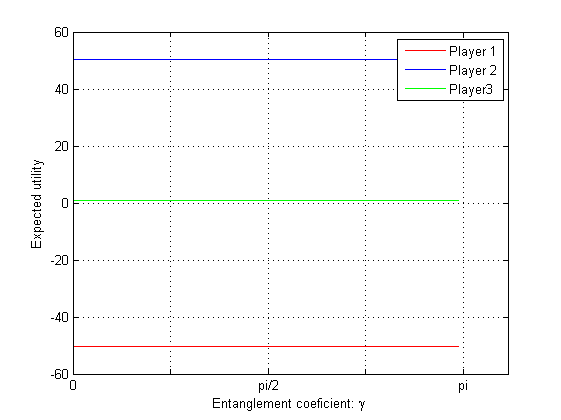
\includegraphics[scale=0.46]{3Rejected99/CDD_DC.PNG}}
    & c1)\putindeepbox[7pt]{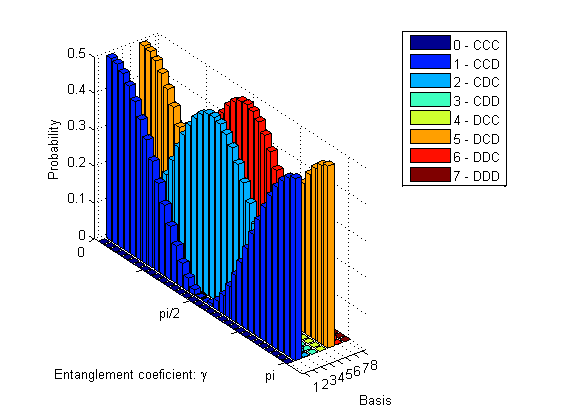
\includegraphics[scale=0.46]{3Rejected99/CDD_DC1.PNG}} \\
\end{tabular}
\caption{c) Expected utility for $3$ players, where the players will use the $(Cooperate , Defect, Defect)$ operators in the first round of the game; in the second round player 2 and player 3 will play $(DC)$. }
\label{tab:3playerCDD_DC99}
\end{center}
 \end{table}

\begin{table}[h]
\begin{center}
\begin{tabular}{cc}
  d)\putindeepbox[7pt]{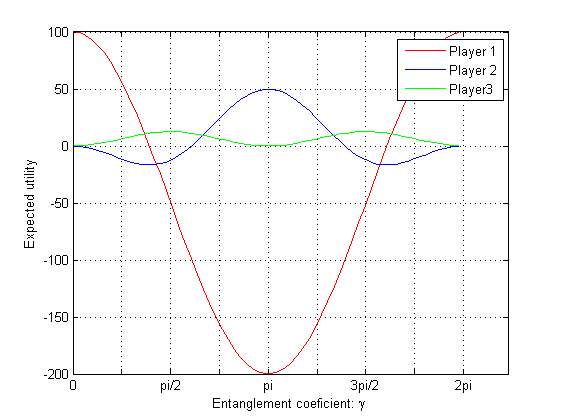
\includegraphics[scale=0.46]{3Rejected99/CDD_DD.PNG}}
    & d1)\putindeepbox[7pt]{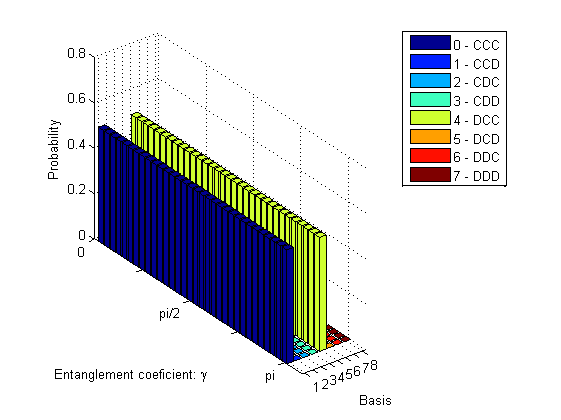
\includegraphics[scale=0.46]{3Rejected99/CDD_DD1.PNG}} \\
\end{tabular}
\caption{b) Expected utility for $3$ players, where the players will use the $(Cooperate , Defect, Defect)$ operators in the first round of the game; in the second round player 2 and player 3 will play $(DD)$. }
\label{tab:3playerCDD_DD99}
\end{center}
 \end{table}


\clearpage
\subsubsection{Initial proposal rejected; $(Defect, Cooperate, Defect)$}

\begin{table}[h]
\begin{center}
\begin{tabular}{cc}
  a)\putindeepbox[7pt]{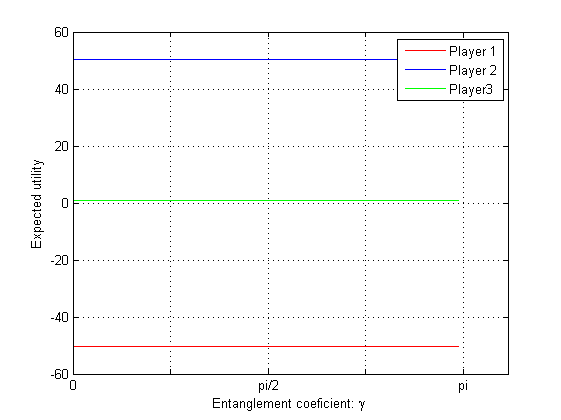
\includegraphics[scale=0.46]{3Rejected99/DCD_CC.PNG}}
    & a1)\putindeepbox[7pt]{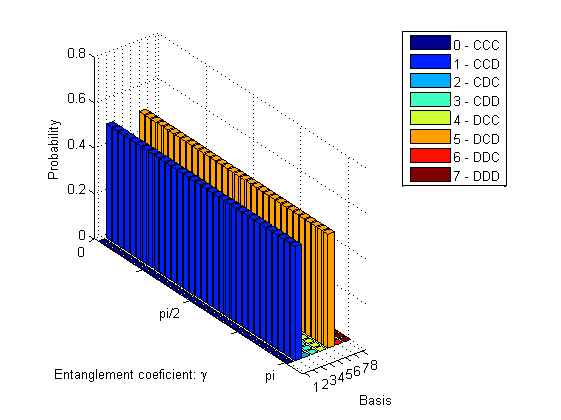
\includegraphics[scale=0.46]{3Rejected99/DCD_CC1.PNG}} \\
\end{tabular}
\caption{a) Expected utility for $3$ players, where the players will use the $(Defect, Cooperate, Defect)$ operators in the first round of the game; in the second round player 2 and player 3 will play $(CC)$. }
\label{tab:3playerDCD_CC99}
\end{center}
 \end{table}

\begin{table}[h]
\begin{center}
\begin{tabular}{cc}
  b)\putindeepbox[7pt]{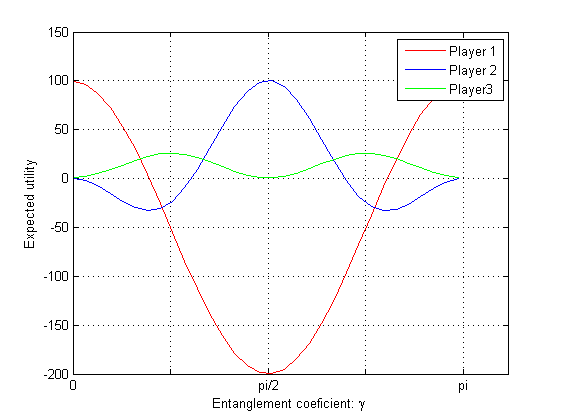
\includegraphics[scale=0.46]{3Rejected99/DCD_CD.PNG}}
    & b1)\putindeepbox[7pt]{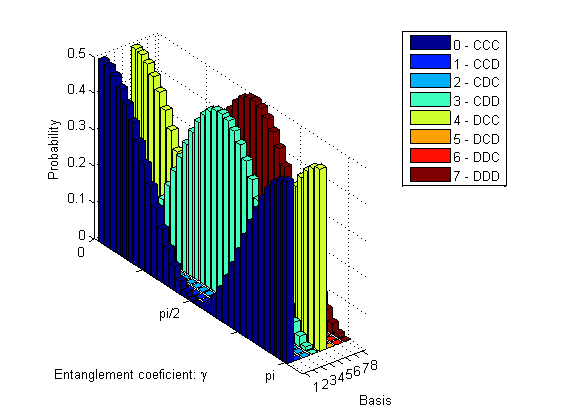
\includegraphics[scale=0.46]{3Rejected99/DCD_CD1.PNG}} \\
\end{tabular}
\caption{b) Expected utility for $3$ players, where the players will use the $(Defect, Cooperate, Defect)$ operators in the first round of the game; in the second round player 2 and player 3 will play $(CD)$. }
\label{tab:3playerDCD_CD99}
\end{center}
 \end{table}

\begin{table}[h]
\begin{center}
\begin{tabular}{cc}
  c)\putindeepbox[7pt]{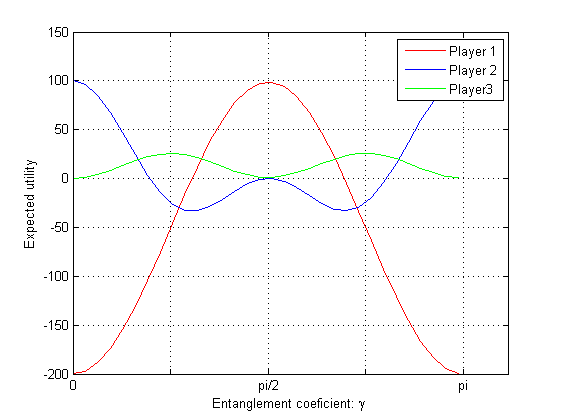
\includegraphics[scale=0.46]{3Rejected99/DCD_DC.PNG}}
    & c1)\putindeepbox[7pt]{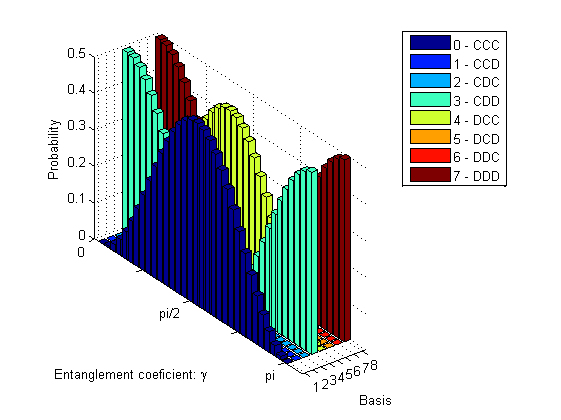
\includegraphics[scale=0.46]{3Rejected99/DCD_DC1.PNG}} \\
\end{tabular}
\caption{c) Expected utility for $3$ players, where the players will use the $(Defect, Cooperate, Defect)$ operators in the first round of the game; in the second round player 2 and player 3 will play $(DC)$. }
\label{tab:3playerDCD_DC99}
\end{center}
 \end{table}

\begin{table}[h]
\begin{center}
\begin{tabular}{cc}
  d)\putindeepbox[7pt]{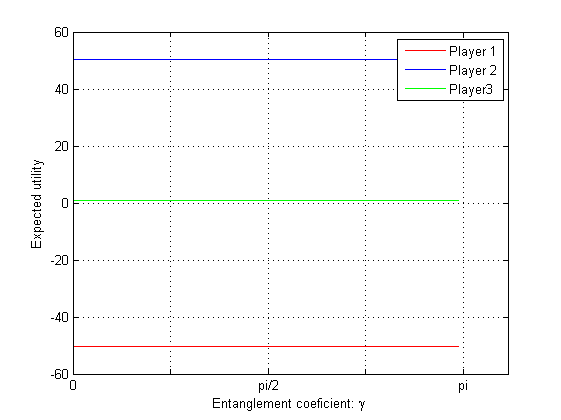
\includegraphics[scale=0.46]{3Rejected99/DCD_DD.PNG}}
    & d1)\putindeepbox[7pt]{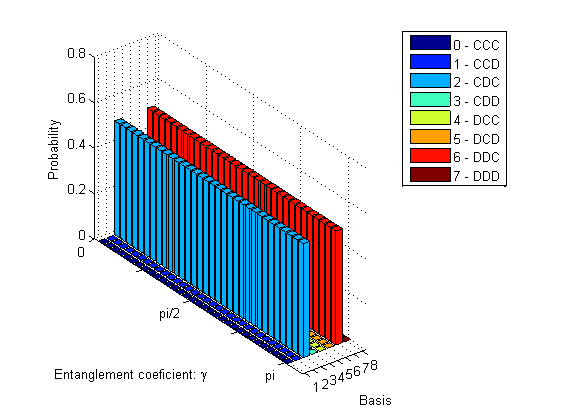
\includegraphics[scale=0.46]{3Rejected99/DCD_DD1.PNG}} \\
\end{tabular}
\caption{b) Expected utility for $3$ players, where the players will use the $(Defect, Cooperate, Defect)$ operators in the first round of the game; in the second round player 2 and player 3 will play $(DD)$. }
\label{tab:3playerDCD_DD99}
\end{center}
 \end{table}

\clearpage
\subsubsection{Initial proposal rejected; $(Defect, Defect, Cooperate)$}

\begin{table}[h]
\begin{center}
\begin{tabular}{cc}
  a)\putindeepbox[7pt]{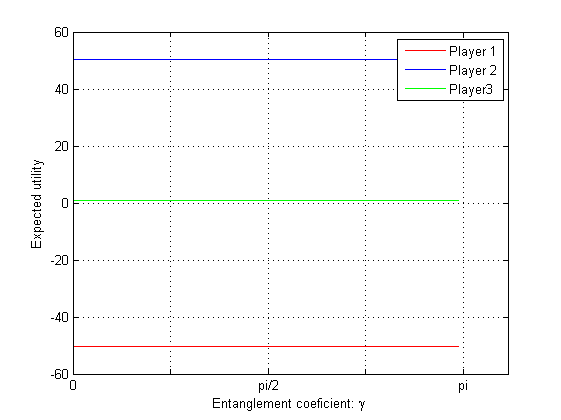
\includegraphics[scale=0.46]{3Rejected99/DDC_CC.PNG}}
    & a1)\putindeepbox[7pt]{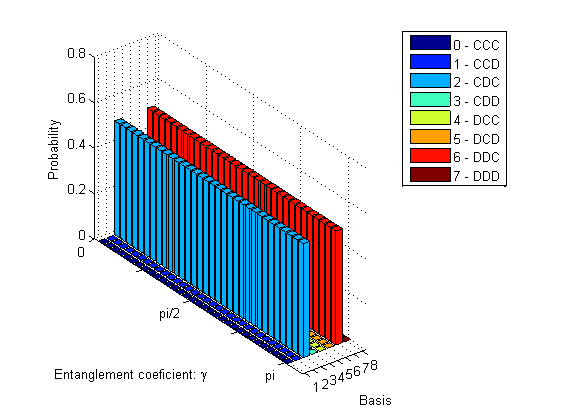
\includegraphics[scale=0.46]{3Rejected99/DDC_CC1.PNG}} \\
\end{tabular}
\caption{a) Expected utility for $3$ players, where the players will use the $(Defect, Defect, Cooperate)$ operators in the first round of the game; in the second round player 2 and player 3 will play $(CC)$. }
\label{tab:3playerDDC_CC99}
\end{center}
 \end{table}

\begin{table}[h]
\begin{center}
\begin{tabular}{cc}
  b)\putindeepbox[7pt]{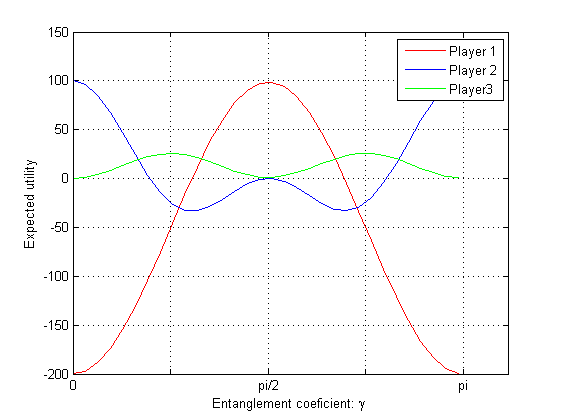
\includegraphics[scale=0.46]{3Rejected99/DDC_CD.PNG}}
    & b1)\putindeepbox[7pt]{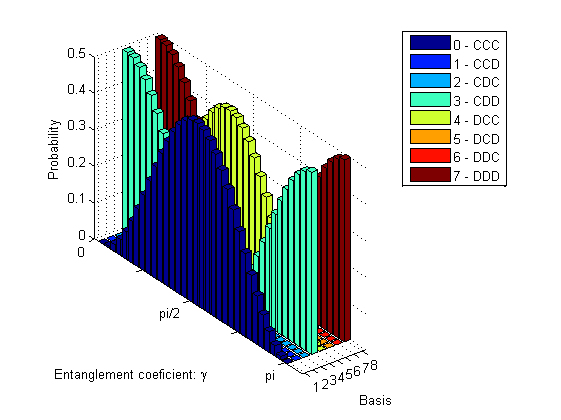
\includegraphics[scale=0.46]{3Rejected99/DDC_CD1.PNG}} \\
\end{tabular}
\caption{b) Expected utility for $3$ players, where the players will use the $(Defect, Defect, Cooperate)$ operators in the first round of the game; in the second round player 2 and player 3 will play $(CD)$. }
\label{tab:3playerDDC_CD99}
\end{center}
 \end{table}

\begin{table}[h]
\begin{center}
\begin{tabular}{cc}
  c)\putindeepbox[7pt]{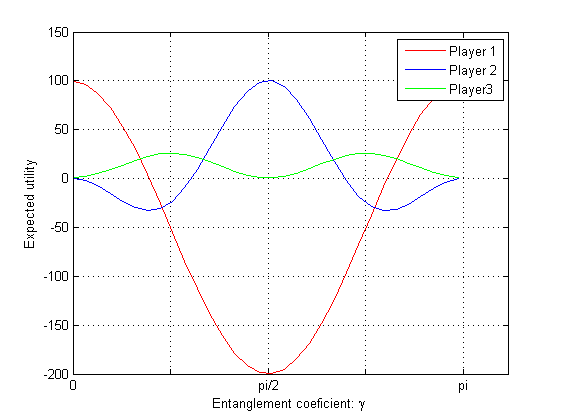
\includegraphics[scale=0.46]{3Rejected99/DDC_DC.PNG}}
    & c1)\putindeepbox[7pt]{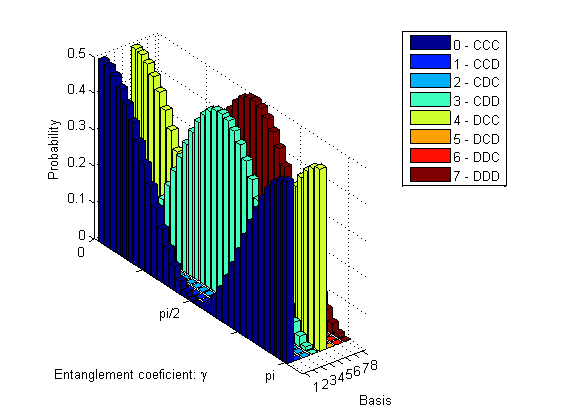
\includegraphics[scale=0.46]{3Rejected99/DDC_DC1.PNG}} \\
\end{tabular}
\caption{c) Expected utility for $3$ players, where the players will use the $(Defect, Defect, Cooperate)$ operators in the first round of the game; in the second round player 2 and player 3 will play $(DC)$. }
\label{tab:3playerDDC_DC99}
\end{center}
 \end{table}

\begin{table}[h]
\begin{center}
\begin{tabular}{cc}
  d)\putindeepbox[7pt]{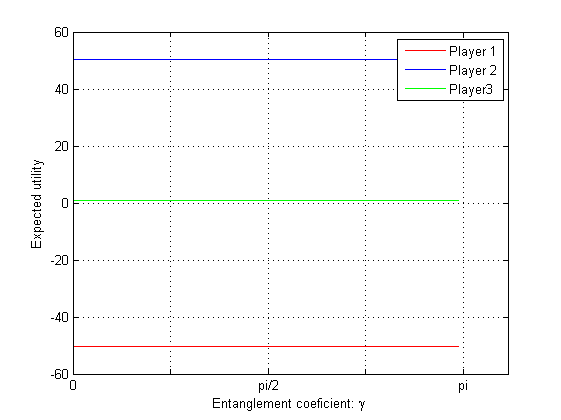
\includegraphics[scale=0.46]{3Rejected99/DDC_DD.PNG}}
    & d1)\putindeepbox[7pt]{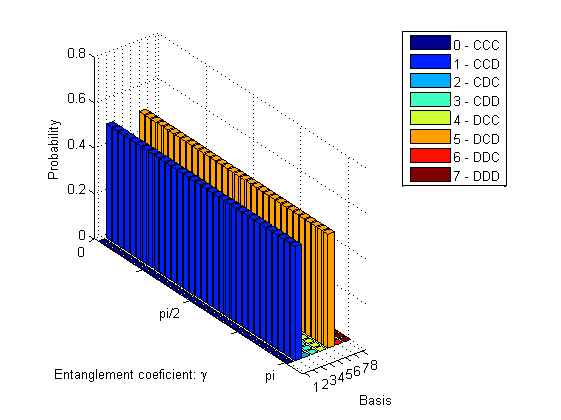
\includegraphics[scale=0.46]{3Rejected99/DDC_DD1.PNG}} \\
\end{tabular}
\caption{b) Expected utility for $3$ players, where the players will use the $(Defect, Defect, Cooperate)$ operators in the first round of the game; in the second round player 2 and player 3 will play $(DD)$. }
\label{tab:3playerDDC_DD99}
\end{center}
 \end{table}

\clearpage
\subsubsection{Initial proposal rejected; $(Defect, Defect, Defect)$}

\begin{table}[h]
\begin{center}
\begin{tabular}{cc}
  a)\putindeepbox[7pt]{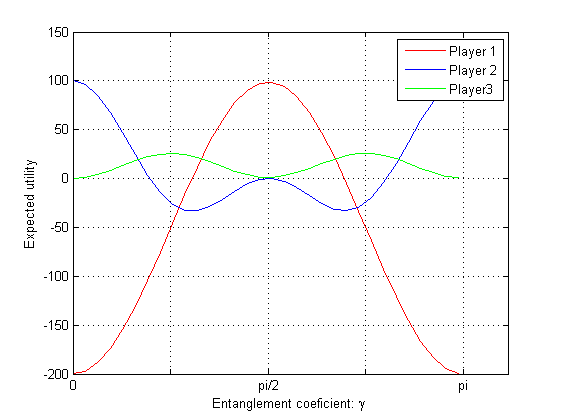
\includegraphics[scale=0.46]{3Rejected99/DDD_CC.PNG}}
    & a1)\putindeepbox[7pt]{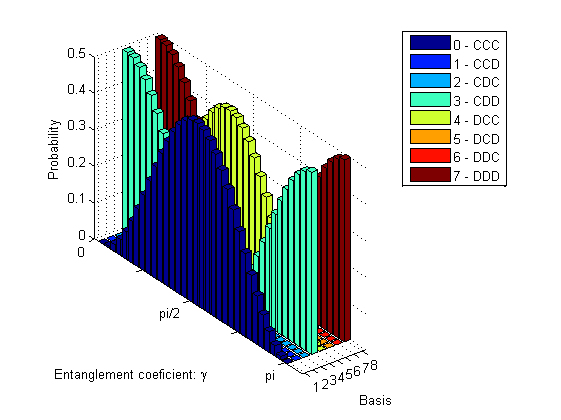
\includegraphics[scale=0.46]{3Rejected99/DDD_CC1.PNG}} \\
\end{tabular}
\caption{a) Expected utility for $3$ players, where the players will use the $(Defect, Defect, Defect)$ operators in the first round of the game; in the second round player 2 and player 3 will play $(CC)$. }
\label{tab:3playerDDD_CC99}
\end{center}
 \end{table}

\begin{table}[h]
\begin{center}
\begin{tabular}{cc}
  b)\putindeepbox[7pt]{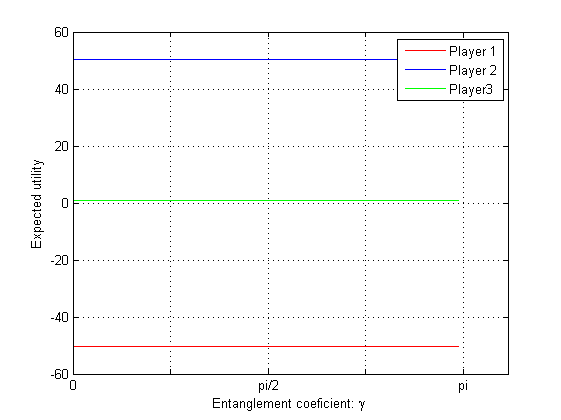
\includegraphics[scale=0.46]{3Rejected99/DDD_CD.PNG}}
    & b1)\putindeepbox[7pt]{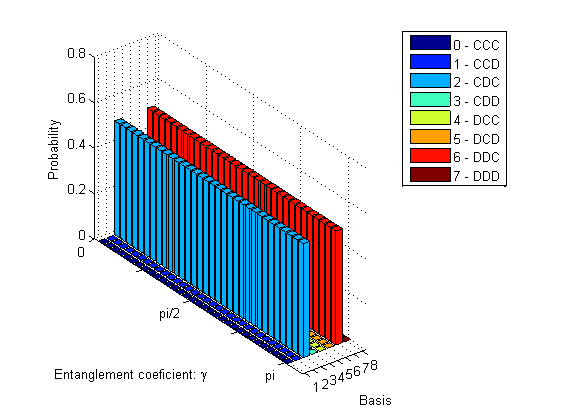
\includegraphics[scale=0.46]{3Rejected99/DDD_CD1.PNG}} \\
\end{tabular}
\caption{b) Expected utility for $3$ players, where the players will use the $(Defect, Defect, Defect)$ operators in the first round of the game; in the second round player 2 and player 3 will play $(CD)$. }
\label{tab:3playerDDD_CD99}
\end{center}
 \end{table}

\begin{table}[ht]
\begin{center}
\begin{tabular}{cc}
  c)\putindeepbox[7pt]{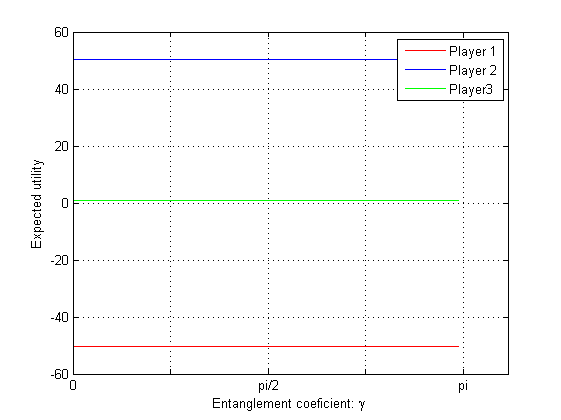
\includegraphics[scale=0.46]{3Rejected99/DDD_DC.PNG}}
    & c1)\putindeepbox[7pt]{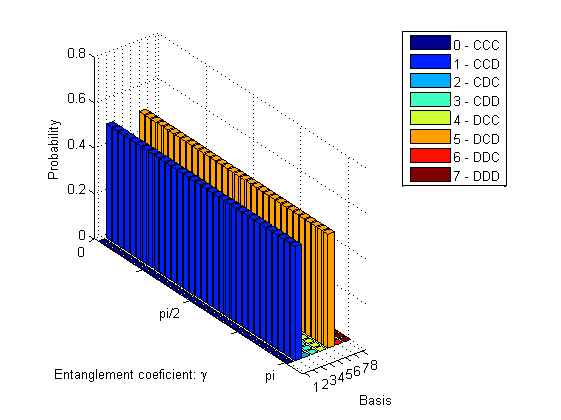
\includegraphics[scale=0.46]{3Rejected99/DDD_DC1.PNG}} \\
\end{tabular}
\caption{c) Expected utility for $3$ players, where the players will use the $(Defect, Defect, Defect)$ operators in the first round of the game; in the second round player 2 and player 3 will play $(DC)$. }
\label{tab:3playerDDD_DC99}
\end{center}
 \end{table}

\begin{table}[h]
\begin{center}
\begin{tabular}{cc}
  d)\putindeepbox[7pt]{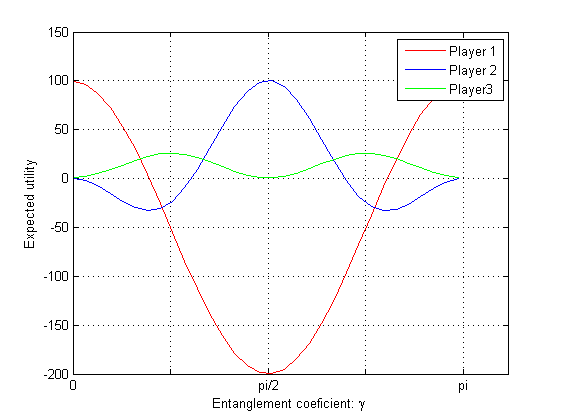
\includegraphics[scale=0.46]{3Rejected99/DDD_DD.PNG}}
    & d1)\putindeepbox[7pt]{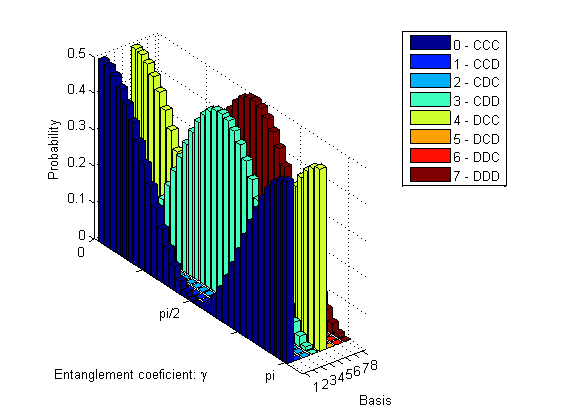
\includegraphics[scale=0.46]{3Rejected99/DDD_DD1.PNG}} \\
\end{tabular}
\caption{b) Expected utility for $3$ players, where the players will use the $(Defect, Defect, Defect)$ operators in the first round of the game; in the second round player 2 and player 3 will play $(DD)$. }
\label{tab:3playerDDD_DD99}
\end{center}
 \end{table}

%\end{itemize}

